\documentclass{article}
% --- watermark (auto-inserted) ---
\usepackage{xcolor}
\usepackage{xfp}% \fpeval; in the kernel since 2022, harmless on older LaTeX
\usepackage{draftwatermark}
\newlength{\watermarkTextWidth}
\AddToHook{begindocument/end}{%
  \SetWatermarkText{\normalfont Generated by The Agentic Scientist}%
  \SetWatermarkFontSize{10pt}%
  \SetWatermarkLightness{0.85}%
  \settowidth{\watermarkTextWidth}{\normalfont\fontsize{10pt}{12pt}\selectfont Generated by The Agentic Scientist}%
  \edef\watermarkScale{\fpeval{0.8 * sqrt(\paperwidth**2 + \paperheight**2) / \watermarkTextWidth}}%
  \edef\watermarkAngle{\fpeval{atand(\paperheight/\paperwidth)}}%
  \SetWatermarkScale{\watermarkScale}%
  \SetWatermarkAngle{\watermarkAngle}%
}
% --- end watermark ---
\usepackage{paper,times}
\usepackage{amsmath,amssymb,booktabs,graphicx,subcaption}
\usepackage{hyperref,url}
\title{Repeatability Is Not Reference Fidelity:\\A Finite-Budget SHAP Audit}
\author{}
\newcommand{\quality}{Q}
\begin{document}
\maketitle

\begin{abstract}
Can one finite-budget SHAP explanation be treated as a reliable account of a fixed tabular prediction? We audit repeated coalition-regression explanations while holding the fitted model, input, and empirical background fixed. The retained evaluation covers German Credit and California ACSIncome, logistic regression, random forests, and gradient boosting, with two fitted seeds and two coalition budgets. We distinguish top-feature repeat agreement, normalized attribution discrepancy against reference values, and efficiency. Aggregate top-three overlap is 0.9459, while reference-fidelity quality is 0.9290; neither is a calibrated reliability probability. Averaging four additional short explanations has lower mean reference quality than one longer explanation at equal coalition count, with an aggregate difference of $-0.03883$. ACSIncome has exact empirical-game references; German Credit has approximate references. These are descriptive results from retained diagnostics marked unverified, not an independent execution audit. They support separate reporting of agreement, fidelity, and cost, rather than a universal deployment verdict or a claim of sampler superiority.
% @evidence[[paper_data.json#/final_evaluation/metrics]]
% @evidence[[paper_data.json#/final_evaluation/evaluation_evidence]]
\end{abstract}

\section{Introduction}
Feature attributions are often presented as a concise reason for an individual prediction. For a trained tabular classifier, however, the prediction may be deterministic while its explanation is not: a finite-budget approximation can return different attribution vectors on repeated calls. This distinction matters when a user sees only a single explanation. A stable list of influential features is useful, but it need not imply accurate attribution magnitudes, and an additive decomposition need not approximate the intended Shapley values closely.

SHAP connects additive explanation with cooperative-game attribution \citep{Shapley1953,Lundberg2017}. Its interpretation depends both on the game being explained and on how that game is approximated. We ask a narrower question than whether explanations are generally trustworthy: \emph{for a fixed fitted classifier, input, and empirical interventional background, what do repeated finite-budget coalition-regression explanations establish about a single returned vector?} We also ask whether spending the same coalition allowance on repeated short explanations is preferable to spending it on one longer explanation. This separates a practical allocation decision from a claim about the general quality of SHAP.

Our central thesis is that repeat agreement, reference fidelity, and computational work must be evaluated separately. The audit measures these quantities on German Credit and ACSIncome across logistic, forest, and boosting classifiers. The reference regime is deliberately explicit: ACSIncome admits complete coalition enumeration, whereas German Credit is compared with independently seeded, higher-budget approximate references. Neither reference regime establishes causal validity. All comparisons concern the probability-scale empirical game, not the correctness of a human-facing rationale.
% @evidence[[paper_data.json#/final_evaluation/evaluation_evidence/episodes]]

The contribution is an auditable comparison framework instantiated with retained attribution vectors and work counters, not a newly certified estimator. It yields three concrete findings. First, high average top-feature agreement coexists with reference-sensitive error, especially in the German Credit conditions. Second, the measured four-short versus one-long allocation contrast is negative on average rather than supporting an averaging recommendation. Third, comparison with package Kernel SHAP changes across datasets and budgets, precluding a universal superiority claim for the studied sampler. The evidence also has an important provenance boundary: the detailed retained diagnostics are marked unverified. Reconstructing their arithmetic does not authenticate the executed source, validate unseen controls, or supply missing gate diagnostics.
% @evidence[[derived_summary.json#/cases]]
% @evidence[[paper_data.json#/final_evaluation/evaluation_evidence/candidate_diagnostics_trust]]

\begin{figure}[t]
\centering
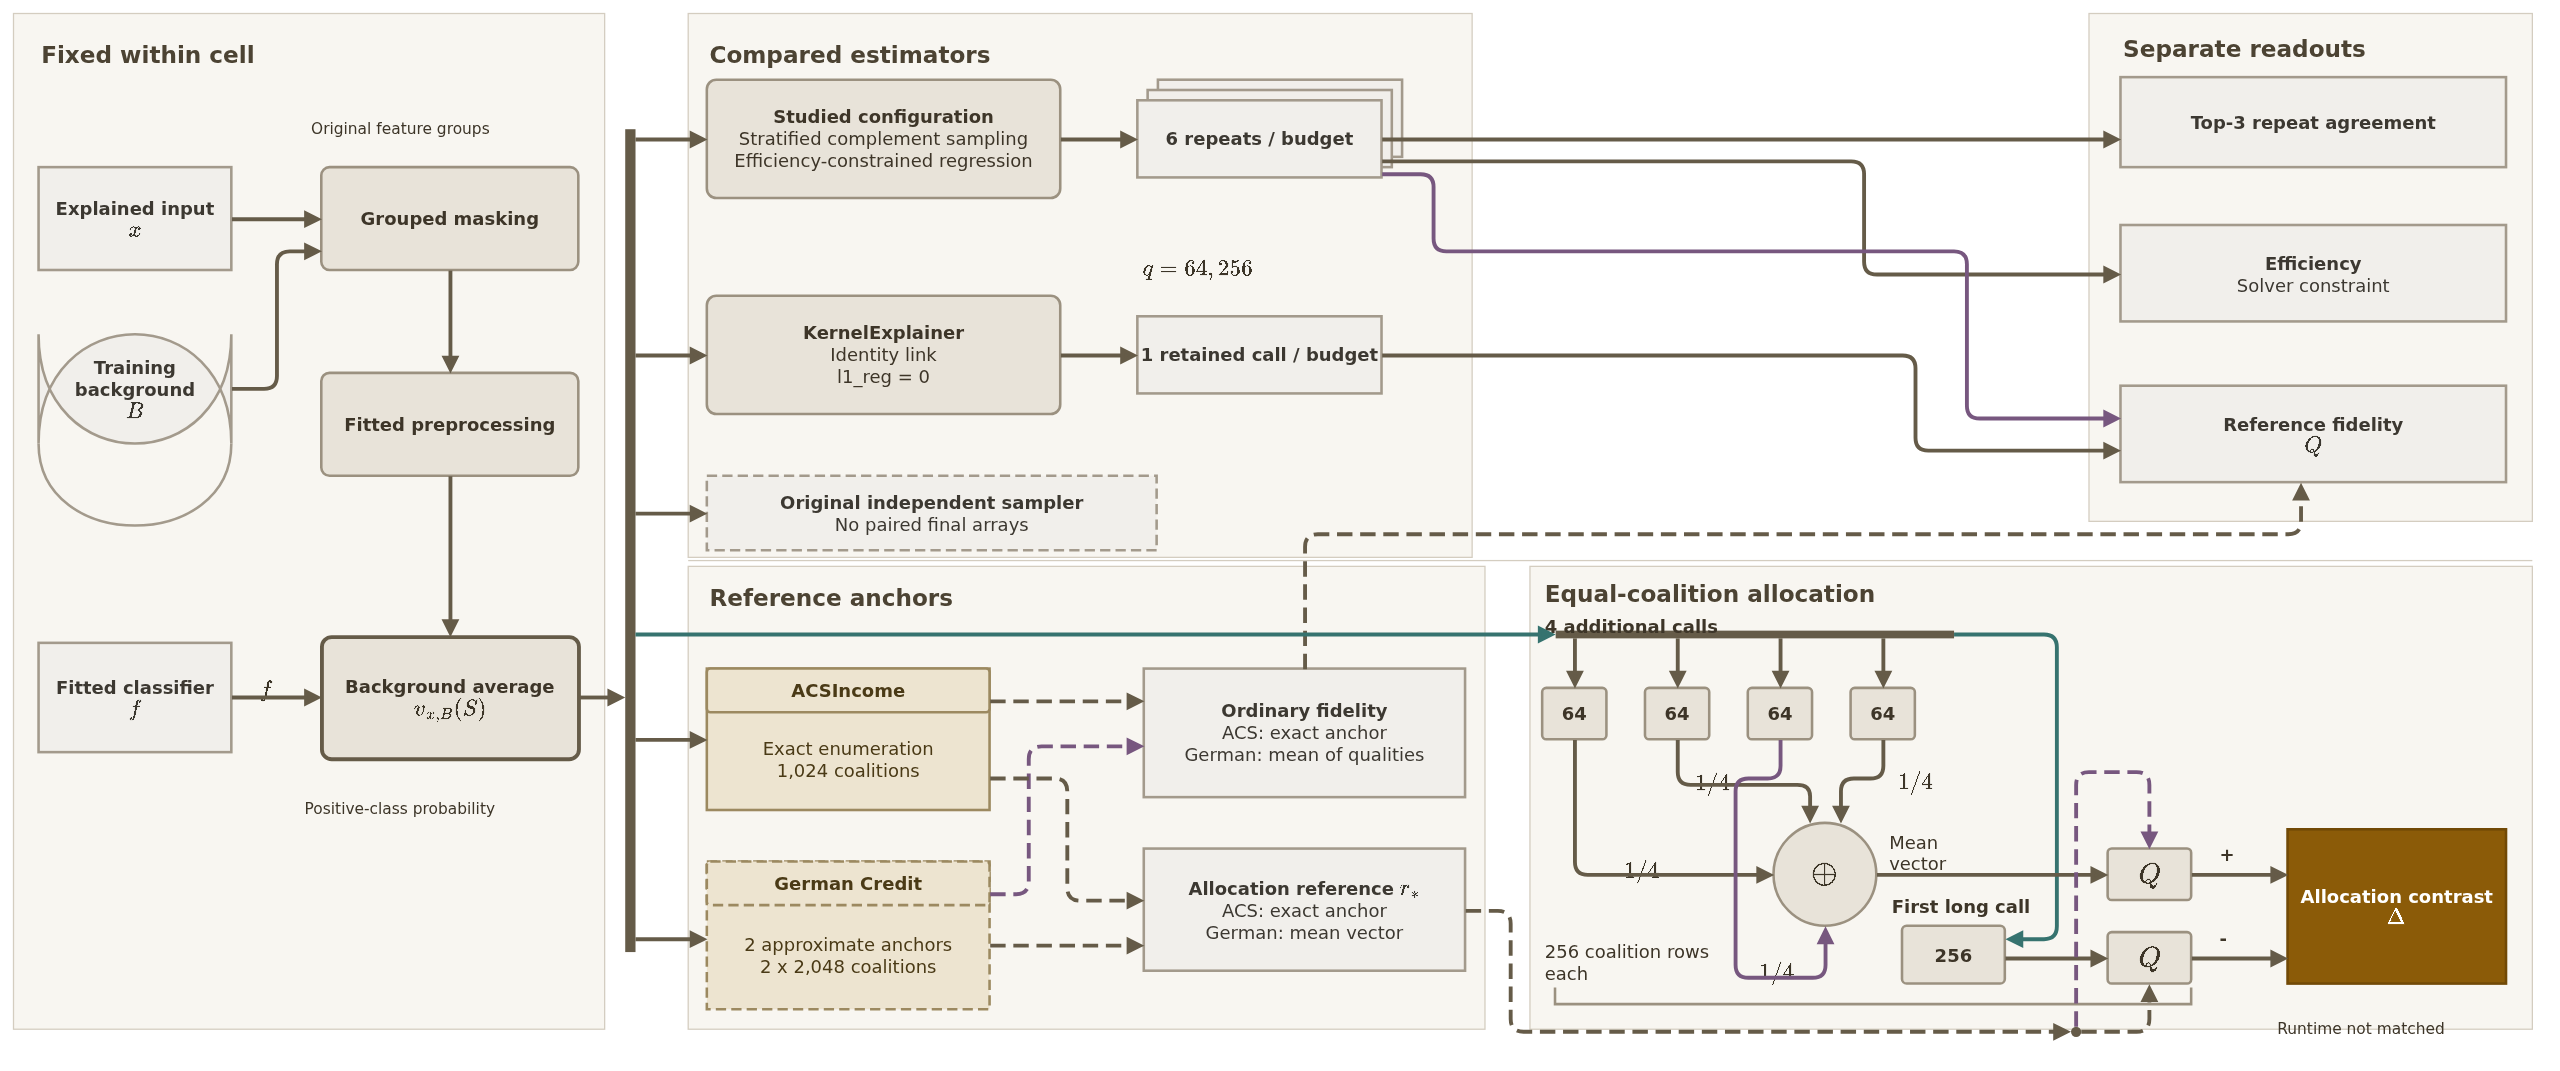
\includegraphics[width=\textwidth,height=1.9in,keepaspectratio]{figures/fixed_game_overview.png}
\caption{Evidence structure of the fixed-game audit. A fixed classifier, input, and empirical background define the target game; repeated explanations, a library comparator, reference anchors, and budget allocation answer different questions. ACSIncome references are exact for that empirical game; German Credit references are approximate. Arrows indicate dependencies, not causal validation. Detailed retained diagnostics are unverified.}
% @evidence[[paper_data.json#/final_evaluation/evaluation_evidence/episodes]]
\label{fig:overview}
\end{figure}

\section{Related Work}
\paragraph{Attribution targets and disagreement.}
The Shapley value allocates a cooperative game's value among its players \citep{Shapley1953}; SHAP uses this structure for feature attribution \citep{Lundberg2017}. Conditional and interventional expectations can answer different questions \citep{Chen2020}. Consequently, disagreement arising from a changed background is not interchangeable with Monte Carlo variation under a fixed game. The permitted study of background-size sensitivity by \citet{Yuan2022} concerns deep models; our within-cell repetitions fix the background and do not reproduce that experiment. Disagreement between explanation methods \citep{Krishna2022} and predictive multiplicity across fitted classifiers \citep{Marx2020} are likewise distinct from repeated approximation of one fixed model prediction.

\paragraph{Sampling and uncertainty.}
Sampling-based Shapley approximation has a substantial methodological literature \citep{Castro2009,Maleki2013,Mitchell2022}. Regression-based estimation can be studied through its bias, variance, and uncertainty \citep{Covert2021}; leverage-score sampling provides another route to approximation guarantees \citep{Musco2024}. These works motivate attention to sampling design and reference error, but their guarantees do not automatically transfer to the dependent finite designs described here. We do not implement leverage-score sampling or run a permutation-estimator comparison. The empirical allocation contrast is therefore about the evaluated configurations, not a test of every variance-reduction method.

\paragraph{What stability measures capture.}
Feature-selection stability can be assessed with chance correction and uncertainty \citep{Nogueira2018}. Ranking comparisons can instead emphasize displacement \citep{Diaconis1977} or preferentially weight early ranks \citep{Webber2010}. We retain the audit's raw top-three overlap and supplementary rank/sign measures rather than substituting an unmeasured stability statistic. These views preserve different information: overlap discards magnitudes, while normalized vector discrepancy remains sensitive to them. Our contribution is the scoped empirical juxtaposition of these readouts and a matched coalition-allocation comparison, without claiming an exhaustive literature review or priority for repeated-explanation evaluation.

\section{Method}
\subsection{Fixed empirical game and research questions}
Let $f(x)$ be the fitted classifier's positive-class probability, let $x$ be an explained input, and let $B=\{b_1,\ldots,b_m\}$ be a fixed training-background sample. Original input columns, including categorical columns before encoding, are the players $D$. The empirical interventional game is
\begin{equation}
v_{x,B}(S)=\frac{1}{m}\sum_{j=1}^{m} f(x_S,b_{j,D\setminus S}),\qquad S\subseteq D.
\label{eq:game}
\end{equation}
The model's fitted preprocessing is applied after masking. Thus a categorical feature is replaced as one group rather than as separately masked indicator columns. The attribution target is the Shapley vector of this game:
\begin{equation}
\phi_i=\sum_{S\subseteq D\setminus\{i\}}
\frac{|S|!(d-|S|-1)!}{d!}\{v_{x,B}(S\cup\{i\})-v_{x,B}(S)\}.
\label{eq:shapley}
\end{equation}
This target is an explanation of $f$ relative to $B$, not a causal effect or a conditional expectation under the population distribution. Increasing background size changes the finite game as well as computational cost. We average results across background sizes for reporting, not because those games have identical attribution targets.
% @evidence[[source_evidence/evaluation/evaluate_final.py#L582]]

We examine three descriptive questions: whether repeated estimates retain the same influential features; how close estimates lie to reference attribution vectors; and whether averaging several short estimates improves fidelity relative to one longer estimate at equal coalition count. A plausible rationale for averaging is variance reduction across independent streams. A competing consideration is that each short regression has fewer design rows and separately pays endpoint overhead. The retained comparison resolves only their combined measured effect; it does not isolate regression conditioning, bias, or complement pairing as the cause.

\subsection{Coalition-regression configuration and comparators}
The readable studied configuration samples coalition sizes according to the Shapley-kernel marginal, with uniform feature subsets conditional on size. For an interior coalition of size $s$, the size mass is proportional to $[s(d-s)]^{-1}$. The source combines complementary sizes into unordered strata with weights proportional to $2/[s(d-s)]$, except for the central stratum when $d$ is even. Randomized stratification allocates size draws, and sampled complement pairs are covered without reuse within a stratum until its finite population is exhausted. Random orientation maintains feature symmetry. These are dependent rows within an explanation, not independent coalition draws.
% @evidence[[source_evidence/downstream/program/src/program.py#L49]]

For total coalition budget $q$, the empty and full masks consume two rows. Writing $n=q-2$, the source assigns
\begin{equation}
p=\min\{\lfloor n/2\rfloor,\max(0,n-2(d-1))\}
\label{eq:pairs}
\end{equation}
complement pairs, with remaining rows sampled individually. Complementary rows are opposite directions in the constrained regression; pairing alone does not double contrast rank. This cap preserves potential design-direction headroom, not a guarantee of full rank or an attribution-error bound.
% @evidence[[source_evidence/downstream/program/src/program.py#L89]]

The solver eliminates the last coefficient using efficiency. For interior mask $z_t$, define $a_{ti}=z_{ti}-z_{td}$ for $i<d$, $T=v(D)-v(\varnothing)$, and $y_t=v(z_t)-v(\varnothing)-z_{td}T$. It solves
\begin{equation}
\widehat\phi_{1:d-1}=\arg\min_u\|Au-y\|_2^2,
\qquad \widehat\phi_d=T-\sum_{i<d}\widehat\phi_i.
\label{eq:regression}
\end{equation}
The readable implementation uses equal-weight least squares with pseudoinverse cutoff \texttt{rcond=1e-10}. Kernel weighting enters through the sampling distribution, not additional regression weights. Enforced efficiency is therefore a construction property, not an independent accuracy test.
% @evidence[[source_evidence/downstream/program/src/program.py#L141]]

Two comparators have different evidentiary roles. The supplied original sampler uses independent kernel-size/subset draws with the same constrained solver; it is a methodological baseline but has no retained paired final attribution arrays for a numerical comparison here. The measured final comparator is \texttt{shap.KernelExplainer}, with identity link, \texttt{l1\_reg=0}, and interior sample request $q-2$. Its stored vectors permit a direct descriptive comparison, but it is not the original independent sampler. Differences between complete configurations do not identify the causal effect of a single sampling component.
% @evidence[[source_evidence/downstream/baseline/src/program.py#L58]]
% @evidence[[source_evidence/evaluation/evaluate_final.py#L595]]

The source snapshot is readable and relevant to the supplied configuration, but its recorded tree identity is not independently authenticated as the exact sealed executable. Accordingly, the implementation description above is source-scoped; the results below describe retained evaluated vectors. Source resemblance and matching aggregate arithmetic do not close this identity gap.
% @evidence[[paper_data.json#/downstream_study/program_tree_sha256]]
% @evidence[[paper_data.json#/final_evaluation/program_tree_sha256]]

\subsection{Data, fitted models, and repeated-explanation protocol}
The public datasets are UCI German Credit \citep{GermanCredit} and California ACSIncome constructed with \texttt{folktables} \citep{Ding2021}. The supplied manifest identifies the latter as the annual ACS PUMS release described in the supplement. Table~\ref{tab:scope} gives the measured evaluation scope. Identical raw and harmonized predictor records are grouped before deterministic content-hash partitioning; the final partition is separated from development data. Hash-based assignment is not guaranteed class stratification. The supplied manifest reports no content overlap between partitions. Training, validation, and explanation pools are distinct.
% @evidence[[source_evidence/evaluation/manifest.json#/partition]]
% @evidence[[source_evidence/evaluation/manifest.json#/content_overlap]]

\begin{table}[t]
\centering
\caption{Retained scientific scope, excluding deterministic replay. A cell fixes one fitted model, explained input, and background. Six repetitions are available at each coalition budget; the allocation comparison uses four additional short calls. Reference budgets include endpoints.}
\label{tab:scope}
\small
\begin{tabular}{@{}lll@{}}
\toprule
Setting & German Credit & ACSIncome\\
\midrule
Original feature groups & 20 & 10\\
Training / validation / explanation pool & 356 / 125 / 131 & 10,000 / 3,000 / 3,000\\
Classifier families & \multicolumn{2}{l}{Logistic, random forest, gradient boosting}\\
Fitted seeds & \multicolumn{2}{l}{7301 and 9109, shown separately}\\
Explained inputs per fit / family & 12 & 12\\
Background rows / coalition budgets & \multicolumn{2}{l}{8 or 32 / 64 or 256}\\
Repetitions per cell and budget & 6 & 6\\
Reference anchors & Two 2,048-budget estimates & Exact 1,024 coalitions\\
\bottomrule
\end{tabular}
% @evidence[[paper_data.json#/final_evaluation/evaluation_evidence/episodes]]
% @evidence[[source_evidence/evaluation/evaluate_final.py#L1000]]
\end{table}

Each classifier is fitted afresh for each statistical seed. Numeric columns receive training-only median imputation and standardization; categorical columns receive dense one-hot encoding with unknown categories ignored. Logistic regression uses $C=1$ and a maximum of 200 iterations. The forest has 64 trees, depth at most 6, and one fitting thread; boosting uses 64 estimators with depth 3. These conventional tree ensembles \citep{Breiman2001,Friedman2001} provide model-family diversity without a neural-network experiment. Broader tabular architecture comparisons \citep{Gorishniy2021} motivate that missing coverage, not a claim of transfer to those architectures.
% @evidence[[source_evidence/evaluation/evaluate_final.py#L625]]

Explained inputs alternate labels and cover ordered predicted-probability positions within each label stratum, rather than constituting a random deployment sample. Backgrounds are nested prefixes of a seeded permutation of training rows. Within each model/input/background cell, repetitions differ only in explainer stream. The study contains 12 fitted dataset/model conditions and 288 input/background cells. A terminal deterministic replay checks reproducibility but is excluded from scientific means and sample sizes. Synthetic constant, copied-feature, and feature-permutation controls are functional checks, not additional public datasets.
% @evidence[[source_evidence/evaluation/evaluate_final.py#L646]]
% @evidence[[derived_summary.json#/cells]]
% @evidence[[paper_data.json#/final_evaluation/evaluation_evidence/episodes]]

Development selected a frozen configuration without establishing an improvement over the original sampler. Development scores are not final reliability measurements. Independently, the reported final evaluation completed and met its qualification requirements. This completion result is not a general-validity or deployment-safety certificate. More importantly, the retained detailed diagnostics are explicitly marked \emph{unverified}; their use here is a transparent descriptive analysis, not independent validation of their provenance. Missing gate-level diagnostics remain unknown.
% @evidence[[paper_data.json#/downstream_study/investigation_outcome]]
% @evidence[[paper_data.json#/grounding_sources/final.qualification.status]]
% @evidence[[paper_data.json#/grounding_sources/final.qualification.outcome]]
% @evidence[[paper_data.json#/final_evaluation/evaluation_evidence/candidate_diagnostics_trust]]

\subsection{Metrics, references, and uncertainty}
Let $H_k(a)$ select the $k=\min(3,d)$ largest absolute entries of vector $a$, breaking ties by stable feature index. Repeat agreement is $|H_k(a)\cap H_k(b)|/k$, averaged across all unordered repeat pairs within a budget. This raw overlap is not chance-corrected and cannot be interpreted as the probability that a returned explanation is reliable. Supplementary rank and sign agreement preserve complementary information.
% @evidence[[source_evidence/evaluation/evaluate_final.py#L789]]

For vector $a$ and reference $r$, define the retained bounded discrepancy quality
\begin{equation}
\quality(a,r)=\left(1+\frac{\|a-r\|_1}{\max(10^{-8},\|r\|_1)}\right)^{-1}.
\label{eq:quality}
\end{equation}
Larger values indicate less normalized error; this is a transformation, not a calibrated probability or an application acceptability threshold. Small reference norms can amplify normalized error. For ACSIncome, ordinary fidelity is $\quality(a,\phi^{\rm exact})$ using enumeration of every coalition. For German Credit it is $\{\quality(a,r_1)+\quality(a,r_2)\}/2$, using two independently seeded higher-budget package estimates. Reference resolution is the separate diagnostic $\quality(r_1,r_2)$; agreement between approximate references does not exclude shared error. The efficiency quality is $(1+|\sum_i a_i-T|/10^{-6})^{-1}$.
% @evidence[[source_evidence/evaluation/evaluate_final.py#L785]]
% @evidence[[source_evidence/evaluation/evaluate_final.py#L825]]

The distinction between these diagnostics is structural. Adding a zero-sum perturbation to an attribution vector preserves efficiency while potentially changing every coordinate. Likewise, perturbations that preserve the leading absolute-feature set leave top-feature overlap unchanged even when attribution magnitudes differ. These observations explain why an efficiency check or repeated feature selection cannot replace Equation~\ref{eq:quality}. They are consequences of the metric definitions, not additional measured controls. Reference fidelity still requires a defensible target: a vector can be close to an empirical-game reference without describing conditional dependence or a causal intervention in the underlying population.
% @evidence[[source_evidence/evaluation/evaluate_final.py#L785]]

The allocation contrast is
\begin{equation}
\Delta=\quality\left(\frac{1}{4}\sum_{j=1}^{4}a^{\rm additional}_{64,j},r_*\right)
-\quality(a_{256,1},r_*),
\label{eq:allocation}
\end{equation}
where $r_*$ is exact for ACSIncome and $(r_1+r_2)/2$ for German Credit. Thus German allocation and ordinary fidelity use different, explicitly defined reference reductions. The short estimates are additional independent streams, not a subset selected from the six reported repetitions. The long estimate is the first retained long call, not the best one. Both choices spend 256 coalition rows. Repeated endpoints, distinct design coverage, and multiple-call overhead differ; equal coalition count is not equal runtime.
% @evidence[[source_evidence/evaluation/evaluate_final.py#L840]]

All reported case means give equal weight to inputs, backgrounds, and relevant budgets; balanced case means are then averaged over datasets, families, and fitted seeds. We preserve the stored descriptive 95\% percentile intervals obtained by resampling explained-input clusters within each fitted condition, using 200 bootstrap draws. Each cluster retains its backgrounds and repeat summaries. Bootstrap methodology \citep{Efron1979,DiCiccio1996} does not turn these few, deliberately selected inputs into a population sample. Repeat pairs are dependent, and the two fits do not justify a population-level training-uncertainty interval. Budget-specific comparisons below have no fabricated confidence bars.
% @evidence[[source_evidence/evaluation/evaluate_final.py#L860]]

\section{Results}
\subsection{Repeat agreement and fidelity answer different questions}
Across retained scientific cells, mean top-three overlap is 0.9458719 and mean fidelity quality is 0.9289531. Efficiency quality is 0.9999999999999954, consistent with a solver that imposes efficiency. These aggregates summarize distinct quantities: subtracting overlap from fidelity is not an error decomposition, and neither value identifies a fraction of acceptable explanations. The decisive evidence is their condition-specific behavior, shown in Figure~\ref{fig:agreement}, together with the definition of each readout.
% @evidence[[paper_data.json#/final_evaluation/metrics]]

\begin{figure}[t]
\centering
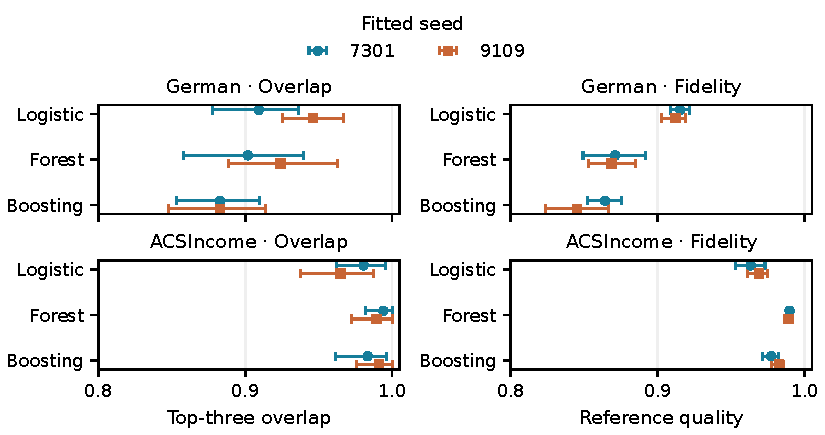
\includegraphics[width=\textwidth]{figures/agreement_and_reference_fidelity.pdf}
\caption{Repeat agreement (left) and reference fidelity (right), by dataset (rows). Points show fitted seeds separately; horizontal bars are stored descriptive 95\% explained-input-cluster bootstrap intervals. Means and intervals pool the same background sizes and budgets within each fit. German Credit uses two approximate anchors; ACSIncome uses exact empirical-game attribution. The axes share a numerical range for readability, not a common probabilistic interpretation.}
% @evidence[[derived_summary.json#/cases]]
\label{fig:agreement}
\end{figure}

German Credit's mean fidelity ranges from 0.8453 to 0.9153 across the displayed fitted conditions, whereas ACSIncome ranges from 0.9632 to 0.9897. German forest overlap is 0.9019 and 0.9241 for the two fits, but its fidelity is 0.8710 and 0.8685. These observations show why a repeatedly selected top-feature set is not a substitute for reference-sensitive magnitude assessment. They do not establish that dimensionality, dataset identity, model complexity, or a particular feature caused the discrepancy: those factors were not independently controlled.
% @evidence[[derived_summary.json#/cases]]

For ACSIncome, exact enumeration makes the discrepancy an error relative to a precisely defined finite game. For German Credit, residual uncertainty in the approximate anchors remains. Approximate-reference agreement within German Credit is high, but its case means range from 0.9801 to 0.9910 rather than proving convergence. A high reference-agreement diagnostic cannot exclude shared bias from the same reference estimator. Conversely, the larger observed German discrepancy should not be reinterpreted as a demonstrated failure of the original sampler, which lacks paired final arrays here.
% @evidence[[derived_summary.json#/cases]]

These results are consistent with a conditional reading of single-call reliability: the retained ACSIncome configurations exhibit close reference agreement on average, while the German Credit conditions warrant more caution, particularly at the smaller budget. They do not supply an acceptance rule for an individual decision. Averages can hide an unstable input, top-feature ties can change overlap with little magnitude change, and probability-scale fidelity does not measure whether a user would act differently.

\subsection{Averaging short calls does not improve the measured allocation contrast}
The aggregate four-short minus one-long quality difference is $-0.0388335$. All 12 fitted dataset/model means are negative. German Credit differences span $-0.1067$ to $-0.0526$; ACSIncome differences span $-0.0078$ to $-0.0018$. Figure~\ref{fig:allocation} retains both fits rather than collapsing their variability into an unsupported across-model confidence interval. Every stored within-fit interval lies below zero, but these are descriptive intervals for the selected explained-input clusters, not a multiplicity-adjusted claim about all tabular models.
% @evidence[[paper_data.json#/final_evaluation/metrics/matched_budget_gain]]
% @evidence[[derived_summary.json#/cases]]

\begin{figure}[t]
\centering
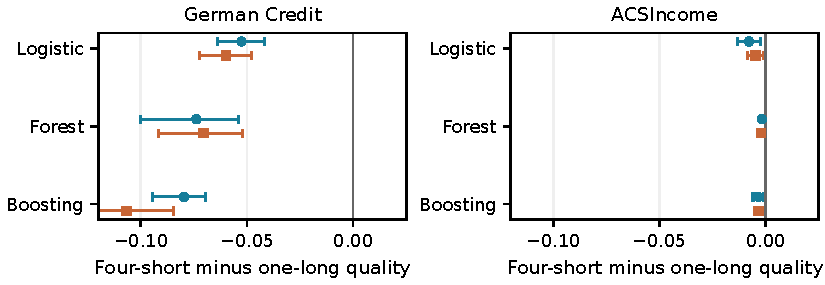
\includegraphics[width=\textwidth]{figures/budget_allocation_contrast.pdf}
\caption{Equal-coalition allocation contrast: quality of the mean of four additional 64-coalition calls minus quality of the first 256-coalition call. Negative values favor the longer call for this comparison. Colors and markers follow Figure~\ref{fig:agreement}. Bars are stored descriptive within-fit input-cluster intervals. German Credit uses the mean approximate reference vector here, not the mean of two fidelity qualities. No causal mechanism or universal loss is identified.}
% @evidence[[derived_summary.json#/cases]]
\label{fig:allocation}
\end{figure}

The comparison directly rejects an empirical recommendation to average four short calls \emph{for this tested allocation and quality metric}. It does not reject averaging in general. In particular, it does not estimate how many short calls would suffice, whether different short budgets would behave similarly, or whether an adaptive stopping procedure would help. The experiment does not isolate whether smaller regressions, dependent design coverage, or another property explains the negative contrast. The matching is of requested coalition rows, including endpoints, not independent observations or arithmetic precision. These distinctions matter because the practical temptation to repeat an inexpensive explanation is not equivalent to improving each regression's information content.

\subsection{Package comparison and budget sensitivity}
Figure~\ref{fig:comparison} compares recorded package calls with the studied configuration. At budget 64, German Credit's package fidelity is higher in each displayed fit/family condition: package means range from 0.8644 to 0.9354, while studied means range from 0.7470 to 0.8593. On ACSIncome at the same nominal budget, studied means range from 0.9474 to 0.9853 and exceed the corresponding package means. The direction therefore depends on the dataset and cannot support a general sampler-superiority claim.
% @evidence[[derived_summary.json#/cases]]

At budget 256, the studied configuration has higher fidelity than at 64 in every displayed fitted condition. German Credit means rise to 0.9436--0.9736; ACSIncome means rise to 0.9791--0.9942. These are within-configuration budget associations, not an isolated ablation of complementary sampling. The package and studied values are often close at the larger budget, with differences of both signs. Only one package attribution per cell and budget is retained, so package seed-to-seed variability cannot be estimated from these records. No budget-specific statistical test is claimed.
% @evidence[[derived_summary.json#/cases]]

\begin{figure}[t]
\centering
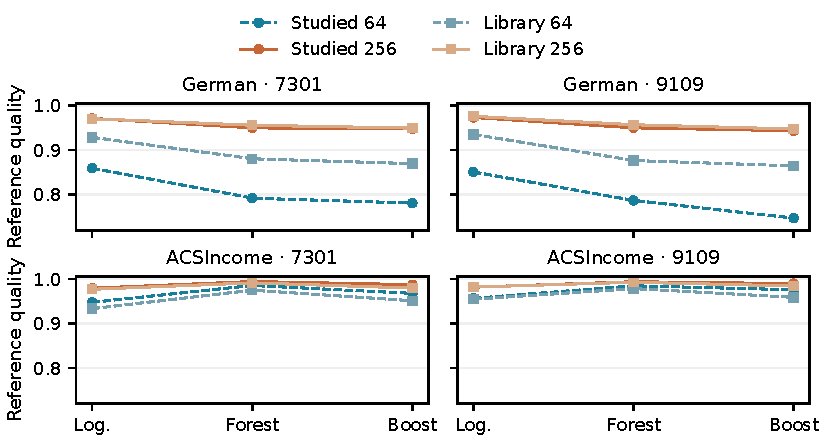
\includegraphics[width=\textwidth]{figures/deployment_estimator_comparison.pdf}
\caption{Reference-fidelity quality by classifier, dataset (rows), fitted seed (columns), and nominal coalition allowance. Studied values average six repeats per input/background cell; library values use the single stored package call in each cell. Lines only connect categorical conditions to aid comparison. No error bars are supplied because budget-specific uncertainty estimates are not retained. The library is not the supplied independent-sampling baseline.}
% @evidence[[derived_summary.json#/cases]]
\label{fig:comparison}
\end{figure}

\subsection{Measured work and the meaning of a budget}
Table~\ref{tab:cost} reports actual prediction-row counters and observed call times rather than equating a sample setting with CPU cost. The studied oracle evaluates every requested mask against every background row, including duplicate and endpoint masks. Hence four short calls and one long call use equal masked-row counts at fixed background size. The package counter differs because its prediction wrapper includes background and explained-input handling; requested coalition budgets do not imply identical prediction-row costs across implementations.
% @evidence[[derived_summary.json#/costs]]
% @evidence[[source_evidence/evaluation/evaluate_final.py#L582]]

\begin{table}[t]
\centering
\caption{Measured work per call, averaged over inputs, fits, and classifier families within each displayed dataset/background/budget condition. Row counts are constant within each condition. Studied time is wall-clock seconds; library time is process CPU seconds. These clocks must not be interpreted as a speedup comparison.}
\label{tab:cost}
\small
\begin{tabular}{@{}lrr rrrr@{}}
\toprule
Dataset & $m$ & $q$ & Studied rows & Library rows & Wall (s) & CPU (s)\\
\midrule
German & 8 & 64 & 512 & 505 & 0.0173 & 0.0198\\
 & 8 & 256 & 2,048 & 2,041 & 0.0563 & 0.0290\\
 & 32 & 64 & 2,048 & 2,017 & 0.0242 & 0.0265\\
 & 32 & 256 & 8,192 & 8,161 & 0.0808 & 0.0573\\
ACSIncome & 8 & 64 & 512 & 505 & 0.0174 & 0.0187\\
 & 8 & 256 & 2,048 & 2,041 & 0.0576 & 0.0280\\
 & 32 & 64 & 2,048 & 2,017 & 0.0248 & 0.0250\\
 & 32 & 256 & 8,192 & 8,161 & 0.0859 & 0.0690\\
\bottomrule
\end{tabular}
% @evidence[[derived_summary.json#/costs]]
\end{table}

Both background length and budget affect work, so background size cannot be treated as a free accuracy adjustment. Reference construction and fitting are separate costs and are not folded into a per-deployment-call timing. The retained record does not establish total campaign CPU consumption; an external resource allowance is not a measured runtime. The budget rationale is consequently modest: evaluate bounded coalition allowances with recorded row counts, preserve reference costs separately, and avoid claiming that the observed wall-clock and CPU counters measure the same resource.

\section{Discussion and Limitations}
\paragraph{A deployment interpretation requires an external tolerance.}
The audit does not identify an application-specific error tolerance, a feature-ranking margin requirement, or a user-action loss. Without these, even a high mean fidelity cannot establish that a single call is an adequate basis for a consequential prediction. The most defensible conclusion is comparative: separate the target game from its approximation, assess repeated top-feature selection and vector error, and specify the resource unit. Agreement can be relevant evidence without being sufficient evidence.

\paragraph{Nonlinear summaries require care.}
The bounded quality transformation compresses large discrepancies, and its average cannot be inverted to recover an average normalized error. In particular, the complement of mean quality is not a measured attribution-error fraction. Pooling across backgrounds and budgets also averages different finite games and computational conditions. A deployment decision would need the distribution relevant to its own fixed game and tolerance, not only the balanced aggregate used here. Our pooled readouts are useful for describing the retained grid, while the separated fits and budget-specific comparisons preserve distinctions that the aggregate hides. They do not identify which new input will be well explained.
% @evidence[[source_evidence/evaluation/evaluate_final.py#L785]]
% @evidence[[derived_summary.json#/cases]]

\paragraph{Reference quality and statistical scope.}
Exact ACSIncome references remove approximation error only for the fixed empirical interventional game. They do not validate background representativeness, preserve conditional feature dependence, or certify causal meaning. German Credit's approximate anchors may share error. The explained inputs are deliberately selected, backgrounds are nested training subsets, and only two fitted seeds are represented. Few input clusters and a small bootstrap ensemble limit interval precision. No new confidence interval across fitted models, deployment distribution, or public datasets is inferred. No isolated component ablation supports causal attribution to pairing or size stratification.

\paragraph{Provenance and completion are distinct.}
The final evaluation is reported as completed and qualified; the absence of a development improvement is not a failed final qualification. Nevertheless, detailed retained diagnostics remain unverified, and the supplied readable implementation is not independently authenticated as the exact sealed source. Recomputing aggregate metrics from stored vectors checks internal arithmetic only. Functional controls and deterministic replay are coarse checks, not a comprehensive execution, adaptivity, or scientific-validity audit. The record does not justify a diagnosis of an unobserved validity failure, nor does it eliminate unknown failure modes.
% @evidence[[paper_data.json#/grounding_sources/final.qualification.outcome]]
% @evidence[[paper_data.json#/final_evaluation/evaluation_evidence/candidate_diagnostics_trust]]

\paragraph{Incomplete coverage is not negative evidence.}
There is no controlled neural-model comparison, conditional-game comparison, background-resampling study, or cross-region/year transfer test. The original independent sampler lacks a paired final comparison. Unavailable measurements are not losses and are not filled with extrapolated values. The observed dataset-dependent comparison and negative allocation result should remain bounded by these omissions. Further empirical coverage would be needed to turn this audit into an operational reliability rule.

\section{Conclusion}
A single finite-budget SHAP explanation cannot be assessed by repeat agreement alone. In the retained fixed-game audit, top-three overlap is high on average, yet reference-sensitive quality varies across datasets, fitted classifiers, and budgets. Enforced efficiency supplies even less evidence of attribution fidelity because it is built into the solver. At equal coalition count, averaging four short explanations has lower mean reference quality than one longer explanation in the evaluated allocation; the data do not establish its causal mechanism or a universal recommendation against averaging.

The useful outcome is a bounded assessment rather than a safety verdict: exact finite-game anchors where feasible, explicitly approximate anchors otherwise, separate agreement and vector-error readouts, input-cluster uncertainty, and measured work counters. Retained diagnostic provenance and source-identity limitations remain unresolved despite arithmetic consistency and reported evaluation completion. The results support closer auditing of a specified explanation configuration, not blanket acceptance or rejection of single-run SHAP in high-risk deployment.
% @evidence[[paper_data.json#/final_evaluation/metrics]]
% @evidence[[paper_data.json#/final_evaluation/evaluation_evidence]]

\clearpage
\bibliography{references}
\bibliographystyle{paper}

\clearpage
\appendix
\section{Supplementary Information}
\subsection{Data provenance and deterministic partitioning}
The data manifest identifies German Credit's UCI archive and California's 2024 one-year ACS PUMS person-record archive. Source URLs, archive/member digests, relationship-code adaptation, and content-grouping rules are retained in \path{source_evidence/evaluation/manifest.json}. German Credit's raw source contains 1,000 records. The ACS source count is 203,591 before the documented processing and caps. These are source counts, not the number of explained decisions. The measured final training/validation/explanation pools are those in Table~\ref{tab:scope}.
% @evidence[[source_evidence/evaluation/manifest.json#/source_urls]]
% @evidence[[source_evidence/evaluation/manifest.json#/source_counts]]

Normalization applies Unicode NFKC, collapsed whitespace, canonical finite decimal numbers, explicit missing markers, and normalized signed zero. Predictor hashes group duplicates before partitioning; original and harmonized predictors are checked separately. A hash prefix assigns development versus final data, and another assigns training, validation, or explanation roles. The final ACS training pool is capped at 10,000 and validation/explanation pools at 3,000. This is a deterministic, source-order-capped partition, not a representative survey subsample. The ACS \texttt{RELSHIPP}-to-\texttt{RELP} adapter is recorded rather than silently treating the columns as identical.
% @evidence[[source_evidence/evaluation/manifest.json#/normalization]]
% @evidence[[source_evidence/evaluation/manifest.json#/partition]]
% @evidence[[source_evidence/evaluation/manifest.json#/relationship_adapter]]

ACS players are \texttt{AGEP, COW, SCHL, MAR, OCCP, POBP, RELP, WKHP, SEX, RAC1P}. Numeric preprocessing covers age and weekly work hours; the remaining columns are categorical. German numeric columns are the zero-indexed positions 1, 4, 7, 10, 12, 15, and 17. The German positive target is the source class coded 2; the ACS target uses the supplied \texttt{ACSIncome} definition. No statistical conclusion about fairness across these attributes is evaluated.
% @evidence[[source_evidence/evaluation/evaluate_final.py#L569]]
% @evidence[[source_evidence/evaluation/evaluate_final.py#L635]]

\subsection{Seeds, uncertainty, and exact aggregation}
Fitted seeds are 7301 and 9109. The source initializes sampler randomness from the fit seed and the call's stream identifier. Higher-budget package references use distinct seeded calls within each input; the deployment package call uses a separate seed offset. Exact references enumerate every subset and sum the weighted marginal contributions in Equation~\ref{eq:shapley}. The ACS game has 10 players, hence 1,024 subsets. Enumeration uses the same empirical background and probability-scale model as the repeated estimates.
% @evidence[[source_evidence/downstream/program/src/program.py#L126]]
% @evidence[[source_evidence/evaluation/evaluate_final.py#L612]]
% @evidence[[source_evidence/evaluation/evaluate_final.py#L662]]

For each cell, repeat agreement averages the 15 unordered pairs among six repeats at each of the two budgets. Fidelity averages the six estimates per budget and then budgets; German fidelity also averages the two reference qualities. All cell metrics are averaged equally within a fitted dataset/model condition. Since all scientific conditions are balanced, equal-weight averaging of the 12 case means reproduces the reported final metrics. The terminal replay is not included in these reductions. Its repeated inputs do not constitute new independent evidence.
% @evidence[[paper_data.json#/final_evaluation/evaluation_evidence/episodes]]
% @evidence[[derived_summary.json#/aggregate]]

The retained bootstrap first averages backgrounds and relevant budgets for each explained input. It resamples these input-level summaries with replacement, using generator seed 812 and 200 draws, and returns the 2.5th and 97.5th percentiles. We do not reuse those pooled intervals as budget-specific bars. Deterministic reconstruction in \path{scripts/build_figures.py} agrees with all stored cell fidelity, overlap, and allocation values to floating-point precision. This establishes consistency of the recorded reductions, not independence or external verification of the inputs.
% @evidence[[source_evidence/evaluation/evaluate_final.py#L860]]
% @evidence[[derived_summary.json#/maximum_reconstruction_error]]

\subsection{Additional retained agreement diagnostics}
Rank agreement is one minus the Spearman-footrule displacement of absolute-attribution rankings divided by $\lfloor d^2/2\rfloor$; ties are stable by feature index. Sign agreement is the fraction of equal coordinate signs after treating magnitudes at most $10^{-8}$ as zero. Table~\ref{tab:diagnostics} reports the deterministic case reductions of the stored pair records. These are supplementary descriptions, not independent tests or alternatives selected to obtain a favorable conclusion.
% @evidence[[source_evidence/evaluation/evaluate_final.py#L789]]

\begin{table}[h]
\centering
\caption{Supplementary mean rank/sign agreement and recorded validation accuracy. Values pool backgrounds, budgets, and repeat pairs within the indicated fitted condition. Validation accuracy concerns predictive performance, not explanation fidelity.}
\label{tab:diagnostics}
\small
\begin{tabular}{@{}llrrrr@{}}
\toprule
Dataset & Family & Seed & Rank & Sign & Accuracy\\
\midrule
German & Logistic & 7301 & 0.8811 & 0.9163 & 0.7680 \\
German & Forest & 7301 & 0.8276 & 0.8728 & 0.7440 \\
German & Boosting & 7301 & 0.8113 & 0.8392 & 0.7200 \\
ACSIncome & Logistic & 7301 & 0.9528 & 0.9803 & 0.8103 \\
ACSIncome & Forest & 7301 & 0.9795 & 0.9781 & 0.7730 \\
ACSIncome & Boosting & 7301 & 0.9567 & 0.9571 & 0.7880 \\
German & Logistic & 9109 & 0.8742 & 0.9117 & 0.7680 \\
German & Forest & 9109 & 0.8076 & 0.8588 & 0.7600 \\
German & Boosting & 9109 & 0.7962 & 0.8311 & 0.7200 \\
ACSIncome & Logistic & 9109 & 0.9511 & 0.9740 & 0.8103 \\
ACSIncome & Forest & 9109 & 0.9744 & 0.9690 & 0.7670 \\
ACSIncome & Boosting & 9109 & 0.9666 & 0.9768 & 0.7880 \\
\bottomrule
\end{tabular}
% @evidence[[derived_summary.json#/cases]]
\end{table}

\subsection{Code locations and evidence boundary}
Readable sampling and regression code is supplied at \path{source_evidence/downstream/program/src/program.py}: size stratification begins at line 51, complement coverage at line 66, design allocation at line 91, and the interface and constrained solver at line 117. The original independent comparator is at \path{source_evidence/downstream/baseline/src/program.py}. The evaluator snapshot at \path{source_evidence/evaluation/evaluate_final.py} defines the empirical-game oracle (line 582), package wrapper (line 595), exact reference (line 612), fitting protocol (line 625), readouts (line 785), and scientific reductions (line 802). These are inspectable substantive sources, not just hashes.
% @evidence[[source_evidence/downstream/program/src/program.py]]
% @evidence[[source_evidence/evaluation/evaluate_final.py]]

The supplied configuration and sealed evaluation carry different recorded tree identifiers. No claim here equates their exact source identity. Detailed final attribution records are retained with an unverified-diagnostics designation. Only the first full query/regression trace per case and additional trace digests are present, not a full raw-mask archive for every call. Checks on the returned regressions and synthetic controls should therefore be read as the reported evaluation protocol, not a comprehensive independent reproduction performed during writing.
% @evidence[[paper_data.json#/downstream_study/program_tree_sha256]]
% @evidence[[paper_data.json#/final_evaluation/program_tree_sha256]]
% @evidence[[paper_data.json#/final_evaluation/evaluation_evidence]]

\subsection{Reproduction, environment, and resource reporting}
The recorded evaluation environment is Python 3.12.15, NumPy 2.2.6 \citep{Harris2020}, SciPy 1.15.3 \citep{Virtanen2020}, pandas 2.2.3 \citep{McKinney2010}, scikit-learn 1.6.1 \citep{Pedregosa2011}, SHAP 0.48.0, and folktables 0.0.12. The source fixes numerical computation to a single CPU core and one numerical-library thread. Dependency pins are in \path{source_evidence/evaluation/requirements.txt}; the resolved environment is in its adjacent manifest. The manuscript uses the official ICLR 2026 review template; template provenance is separate from the older data-resource template snapshot.
% @evidence[[source_evidence/evaluation/manifest.json#/runtime]]
% @evidence[[source_evidence/evaluation/requirements.txt]]
% @evidence[[template_provenance.json]]

\path{REPRODUCING.md} gives commands and limitations. \path{scripts/build_figures.py} reads the immutable evidence registry, reproduces the numerical figure inputs, checks the stored reductions, and exports the quantitative figures as vector PDF and 300-DPI PNG. Table~\ref{tab:scope} is a protocol summary; Table~\ref{tab:cost} reduces retained counters; Table~\ref{tab:diagnostics} is generated from retained pair summaries and accuracy fields. No model training or new evaluation is invoked by the manuscript build. The conceptual overview is reserved for the external figure-rendering workflow and contains no measured result.

Reconstructing the figures from retained records is not the same as rerunning the sealed study. Full evaluation additionally requires the data snapshot and the original execution interface; the evaluator's command-line interface and its resource assumptions are supplied, but a portable replacement execution service is not claimed. Data source URLs and processing rules are documented to support reconstruction, with exact-snapshot equivalence requiring the recorded digests. The final record contains episode wall durations of 222.48 and 194.99 seconds, not a measured end-to-end campaign CPU total. They must not be extrapolated into a complete resource accounting.
% @evidence[[paper_data.json#/final_evaluation/evaluation_evidence/episodes]]

\subsection{LLM Usage}
LLM assistance was used to formulate candidate sampling designs, draft implementation changes, plan the paper, inspect supplied artifacts, write the manuscript and plotting code, curate exact-identifier references, and check consistency. The visible study is synthesized around the measured reliability questions rather than the order of development. No new model evaluation was run during manuscript writing. Generated prose and code are not themselves empirical evidence; quantitative conclusions are restricted to the supplied registry and its explicitly derived artifacts. The retained record does not support assigning unseen human or automated roles beyond this disclosed assistance.

\end{document}
